
\section{Domain Name System}

Das Internet ist ohne die Technologie des \emph{Domain Name Systems}, im folgenden mit DNS abgekürzt, kaum noch vorstellbar. Über diesen Service ist es möglich für den Menschen einfach lesbare, alphabetische Namen, statt mehrstellige Nummern zu nutzen, um Ressourcen in einem Netzwerk aufzurufen und auf diese zuzugreifen. Diese alphanumerischen Namen werden ebenfalls als \emph{Domain Names} bezeichnet. Das Routing in einem großen Netzwerk wie dem Internet wäre jedoch schwer über solche Namen zu realisieren, stattdessen werden hierzu numerische IP-Adressen verwendet. Um trotzdem die besser nutzbaren alphabetischen Ausdrücke nutzen zu können ist also ein Service zur Übersetzung dieser in IP-Adressen gefordert. Früher mussten die IP und der zugehörige Domain Name lokal und manuell in einer Datei namens \textit{hosts} gespeichert werden. Mit dem enormen Wachstums des Internets musste jedoch eine neue Möglichkeit geschaffen werden. Dieses Technologie bezeichnet man als \emph{Domain Name System}. \cite{Schreiner.2016}

Das im vorherigen Absatz beschriebene bedeutet, jedes Mal wenn der Domain Name einer Netzwerkressource, wie eines Webservers, eingegeben wird, muss diese zunächst in das IP-System übersetzt werden. Die Auflösung des Domain Namens kann jedoch nicht durch die reine Übersetzung der Zeichen erfolgen. Die Funktionsweise der Auflösung gleicht mehr der Verwendung eines Telefonbuchs. Auf einem DNS Server ist eine Tabelle hinterlegt. Jede Zeile in dieser Tabelle besteht aus mindestens zwei Werten und wird als Record bezeichnet. Dem Domain Namen und der dazugehörigen IP-Adresse. Wird über einen sogenannten DNS-Lookup ein Domain Name angefragt, kann nun als Antwort die passende IP-Adresse zurückgegeben werden, über welche die erfragte Ressource erreicht werden kann.

\subsection{Domain-Namespace}
Der sogenannte Domain-Namespace (englisch für Namensraum) ist in einer Baumstruktur gegliedert und in unterschiedliche Zonen aufgeteilt. Der Wurzelknoten des Baumes stellt der Root-Knoten dar. Dieser wird durch einen Punkt symbolisiert. An erster Stelle nach dem Root-Knoten stehen die sogenannten Top-Level-Domains (TLD). Die meist verwendetn TLD laut einer Statistik vom Mai 2018 sind \textit{com} für \textit{Commercial} mit 46,5\% und darauf folgend der für Organisation stehende Eintrag \textit{org} mit 5,1\% \cite{w3techs.2018}. Diese Top-Level-Domains werden auch als \textit{generic Top-Level-Domains(gTDL}) bezeichnet, da sie einen länderübergreifenden Code darstellen. Zusätzlich gibt es noch Top-Level-Domains, die einen Ländercode repräsentieren. Die meist verwendete länderspezifische TLD oder auch ccTLD (country code top-level-domain) ist hierbei die russische \textit{ru} und auch die für Deutschland stehende \textit{de} findet häufige Verwendung. \cite{IndianaUniversity.14.05.2018} 

Die Second-Level-Domain (SLD) befindet sich hierarchisch unter der Ebene der TLD. Sie wird häufig als frei wählbarer Name der Domain bezeichnet. Die einzelnen Hierarchiestufen werden von unten nach oben geschrieben und durch einen Punkt getrennt. Diese Schreibweise wird auch als \textit{Fully-Qualified Host Name} auf deutsch \textit{vollständig angegebener Rechnername}, bezeichnet. Ein Beispiel wäre hierfür die offizielle Adresse der Homepage der Hochschule \textit{fhws.de}, wobei fhws die SLD darstellt. Der Punkt, welcher den Root-Knoten repräsentiert wird meist weggelassen. Die auf die Second-Level-Domain folgenden Ebenen in der Baumstruktur werden auch als Sub-Domains bezeichnet. Diese dienen dem SLD Besitzer meist dazu unterschiedliche Services anzubieten oder eben direkt auf ein Netzwerkgerät zuzugreifen. \cite{Schreiner.2016} \cite{1und1.2018} 

Ein vereinfachtes Beispiel einer solchen Struktur ist in Abbildung \ref{fig:DNSTree} unter Verwendung der Domain \textit{mail.google.com} zu sehen. Diese Domain führt auf den E-Mail Service von Google. Als weiteres Beispiel stellt der Domain-Name \textit{de.wikipedia.org} dar. Nachdem unter \textit{en.wikipedia.org} die englische Version der Wikipedia Website zu finden ist, bietet die Third-Level-Domain \textit{de} in dem Beispiel die Möglichkeit auf die deutsche Variante des Wikipediaangebots zu gelangen.

\begin{figure}[ht]
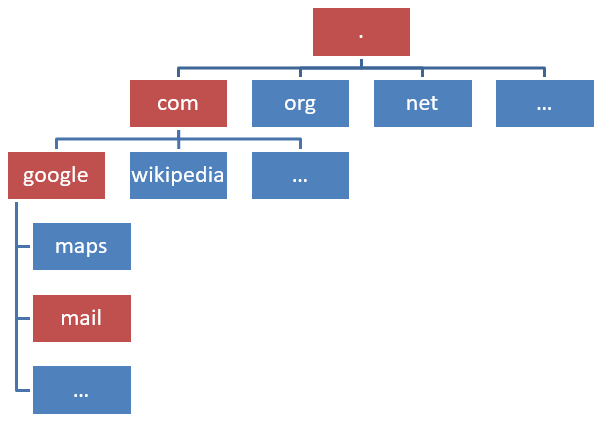
\includegraphics[width=\columnwidth]{images/dnsTree.png}
\caption{Beispiel der Domain mail.google.com in Baumstruktur}
\label{fig:DNSTree}
\end{figure}

\subsection{DNS-Server}
Die Anzahl an Domain-Names ist enorm groß und die Namensauflösung wäre wirtschaftlich kaum über allwissende DNS Server realisierbar. Deshalb ist der Namensraum in unterschiedliche, von einander unabhängige Zonen aufgeteilt und als verteiltes System über mehrere sogenannte Nameserver realisiert. Diese dezentrale Verwaltung des Namensraums ermöglicht eine Lastverteilung und gewährleistet ebenfalls über eine bessere Ausfallsicherheit durch multiple Redundanzen. 

Bei DNS-Servern unterscheidet man zwischen zwei Typen. Jede Zone enthält mindestens einen \textit{Autoritativen DNS-Server}. Dieser repräsentiert seine Zone und verwaltet lediglich orginale und definitive Einträge. Der Autoritative DNS-Server speichert keine Routing Informationen über andere Zonen und liefert nur eine Antwort auf Records die er tatsächlich selbst besitzt. Autoritative DNS-Server sind meist in einem Servercluster organisiert und der Master wird mehrfach durch andere Slave-Nameserver gespiegelt um Lastverteilung und Ausfallsicherheit zu gewährleisten. 

Ein Nicht-autoritativer DNS-Server speichert zuvor durchgeführte DNS-Namensauflösungen. Er enthält nicht nur Informationen zu der Zone in der er sich befindet sondern ebenfalls Datensätze aus zweiter oder dritter Hand. Erhält er eine Anfrage zu einer Domain, zu der er keine Antwort liefern kann, übernimmt der Nameserver die Arbeit der weiteren Namensauflösung. Erhält er den gesuchten Eintrag, gibt er ihn zurück an den Auftraggeber und speichert ihn in seinem Arbeitsspeicher für zukünftige Anfragen. Da sich die Einträge in den fremden Namensräumen jedoch jederzeit verändern können, erhält jeder Eintrag seine eigene Time-to-live. Läuft diese ab wird der Datensatz aus dem Speicher entfernt.  Informationen, welche von einem Nicht-autoritativen DNS-Server gehalten werden, werden auch als \textit{nicht gesichert} angesehen. \cite{1und1.2018}

\subsection{DNS-Lookup}
Der Aufbau des DNS in einem dezentralen Datenbanksystem erschwert die Auflösung im Gegensatz zu einer zentralen Lösung, da die Informationen nicht an einem Ort durch eine einzelne Abfrage gefunden werden können. Wird nun, zum Beispiel durch die Eingabe einer URL in den Browser, ein DNS-Lookup angestoßen, so übernimmt zunächst der Betriebsystem interne Resolver die Aufgabe. Dieser Resolver speichert die zugehörigen IP Adressen zu den angefragten Domain-Names im Cache und liefert der Client-Anwendung den zugehörigen Wert direkt zurück.  Ist der Eintrag nicht im Zwischenspeicher vorzufinden, so wird einen neue Anfrage  an den nächsten DNS-Server weitergeleitet generiert. Befindet sich im eigenen Netzwerk ein Nameserver, so wird dieser die Anfrage versuchen aufzulösen, ansonsten ist als nächste Instanz meist der DNS-Server des Internetproviders eingetragen. Dieser gleicht die Anfrage mit seinen Datenbeständen ab und liefert die angefragte IP-Adresse bei Erfolg zurück an den Resolver. \cite{1und1.22.01.2018}

Kann der gesuchte Datensatz hier nicht gefunden werden kontaktiert der DNS-Server einen Root-Server. Dieser verwaltet wie zuvor beschrieben die Adressen für die TLDs. Der Root-Server kümmert sicher nicht selbst um die weitere Namensauflösung, sondern liefert dem anfragenden Nameserver lediglich einen Hinweis wo der angefragte Eintrag zu finden sein könnte \cite{Schreiner.2016}. Also die IP-Adresse des Nameservers zur gesuchten TLD. Hier ist die Unterscheidung eines iterativen und eines rekursiven Vorgehens der unterschiedlichen DNS-Server zu erkennen. Von Rekursion spricht man dann, wenn der DNS-Server die weitere Namensauflösung übernimmt und selbstständig bei anderen Servern versucht die Information einzuholen. Bei Erfolg wird das Ergebnis zurück an den Resolver geliefert. Bei Iteration beantwortet der DNS-Server lediglich die Anfragen, über die er selbst die Informationen verwaltet. Anstatt selbstständig die Namensauflösung weiter zu verfolgen liefert er lediglich einen Hinweis auf den nächsten anzufragenden Nameserver zurück, der die Informationen halten könnte. Der Resolver muss sich selbst um die weitere Auflösung des Domain-Namens kümmern. \cite{1und1.22.01.2018}

Nachdem der Root-Server die IP-Adresse des zugehörigen TLD-Nameservers an den Resolver weitergegeben hat, kann einen Anfrage an diesen gestellt werden. Der angefragte Server kennt wiederum den Server der die Informationen zur benötigten Domain hält und liefert diesen zurück. Nun kann die letzte Anfrage des Nameservers des Internetproviders gestellt werden. Hat er nun die passende IP-Adresse zur vom Resolver angefragten Domain erhalten, kann diese nun an die ursprüngliche Client-Anwendung weitergegeben werden und im letzten Schritt eine Verbindung zur Ziel-IP hergestellt werden. Hier wird ein weiterer Vorteil des DNS sichtbar. Wird ein Endpunkt, wie ein Webserver, umgezogen, so ändert sich lediglich die IP-Adresse und der Endbenutzer bekommt hiervon nichts mit, da er nur den Domain-Name sieht, welcher gleich geblieben ist. \cite{Schreiner.2016}

\subsection{Time-to-live} \label{lab:ttl}
Die Nicht-autoritativen DNS-Server, welche sich rekursiv um die Auflösung eines Domain-Namens bemüht haben, speichern diesen ermittelten Datensatz jetzt in ihrem Cache. Die Dauer, wie lange die Adresskombination gültig ist wird über die Time-to-Live (TTL) bestimmt. Diese wurde zusammen mit der Information von dem zuständigen Autoritativen DNS-Server mitgegeben. Wird ein Record durch das Ablaufen der TTL ungültig, wird dieser aus dem Zwischenspeicher entfernt. Der TTL-Wert gibt also an, wie schnell die Welt eine Änderung mitbekommen soll. 

Eine kurze TTL würde bedeuten, dass Records aus zweiter oder dritter Hand nur kurze zeit im Cache behalten werden dürfen. Hierbei ist kurz im Bereich von 5 Minuten bis wenige Stunden zu interpretieren. Der Vorteil hiervon ist, dass Änderungen wie ein Serverumzug schnell propagiert werden kann und außerdem den Verkehr bei einer hohen Zielserverauslastung schnell umzulagern auf alternative Server. Auch auf den Ausfall eines Servers kann schneller reagiert werden, da die zwischengespeicherte Information auf den ausgefallenen Server nicht noch über Stunden oder gar Tage als gültige Adresse gilt.

Von einer Langen TTL spricht im Bereich von mehreren Stunden bis Tagen. Eine längere TTL verspricht eine bessere Customer-Experience, da die Latenz für den DNS-Lookup nach dem ersten Mal für eine gewisse Zeit umgangen wird. Ein weiterer Vorteil ist die Reduzierung der Kosten durch niedrigere Netzwerkauslastung und bei der Nutzung eines Cloud-DNS-Services durch die Reduzierung der anfallenden Querries.

Als Best-Practice für den Einsatz von kurzen und langen TTLs hat sich herausgestellt, dass eine höhere TTL meistens sinnvoll ist. Sollte eine Änderung vorgenommen werden, die Einfluss auf das DNS hat, soll nun als Vorbereitung die TTL gesenkt werden. Daraufhin wird einige Zeit abgewartet, bis die kürzere TTL sich durchgesetzt hat. Nach Ablauf der Wartezeit kann nun die Änderung durchgeführt werden. In folge der kürzeren Caching-Zeit werden getätigte Änderungen nun schneller propagiert. Die Tite-to-Live wird nun noch für eine gewisse Zeit niedrig gehalten umd eventuell vorkommenden Problemen entgegenzuwirken oder die Änderungen rückgängig zu machen. Gibt es keine negativen Auffälligkeiten kann nun die TTL erneut auf den ursprünglichen Wert angehoben werden.

\subsection{Root-Nameserver}
Das Domain Name System basiert auf mehreren Root-Servern. Alle dieser Server enthalten die gleichen Informationen und verwalten die Root-Zone. In dieser Zone sind sämtliche gTLDs und ccTLDs hinterlegt. Die Root-Server bilden den zentralen Knoten des Internets. Dabei ist zu erwähnen, dass die meisten dieser Server derzeit in den USA stehen. Sie werden aktuell von den folgenden 12 Behörden verwaltet:
\begin{itemize}
    \item A - VeriSign Global Registry Services
    \item B - University of Southern California - Information Sciences Institute
    \item C - Cogent Communications
    \item D - University of Maryland
    \item E - NASA Ames Research Center
    \item F - Internet Systems Consortium, Inc.
    \item G - U.S. DOD Network Information Center
    \item H - U.S. Army Research Lab
    \item I - Autonomica/NORDUnet
    \item J - VeriSign Global Registry Services
    \item K - RIPE NCC
    \item L - ICANN
    \item M - WIDE Project
\end{itemize}

Erreichbar sind die Root-Nameserver über 13 verschiedenen IP-Adressen. Diese Adressen sind wohl bekannt und werden so selten wie möglich geändert. Jeder DNS-Server erhält die Root-Server-Adressen als Liste fest installiert. Sollte sich die IP eines Root-Servers ändern, arbeitet der DNS-Server mit den verbleibenden 12 funktionierenden Adressen, bis seine Software auf den neuen Stand aktualisiert wird. \cite{NETNOD.2018}

\subsection{Anycast}
Die große und immer weiterwachsende Anzahl an täglichen Anfragen sind jedoch nicht mehr wie früher allein von 13 Servern in einer angemessenen Zeit zu bearbeiten. Deshalb beantworten die 13 Root-Nameserver die DNS-Requests nicht allein, sondern werden im Hintergrund von einer großen Anzahl an Servern beantwortet. Somit sind es mittlerweile mehrere hundert Server, die sich um die Bearbeitung von Root-DNS-Anfragen kümmern. Diese Aufteilung wird jedoch vor den einzelnen Clients verborgen.

Nur wie ist eine solche Aufteilung sinnvoll und ohne zusätzliche Load-Balancer möglich? Hierfür wurde eine Technologie gewählt die als Anycast bezeichnet wird. Bei dieser Technologie erhalten mehrere Endpunkte die gleiche IP-Adresse. Wird nun ein DNS-Request an einen Root-Server gesendet, wird die Anfrage an den Server weitergeleitet, der am nächsten zum anfragenden Client steht. Da nur 3 der Root-Nameserver außerhalb der USA stehen ist somit über eine weitere geographische Verteilung der Server auch eine schnellere Verarbeitung und bessere Lastverteilung weltweit möglich. Ein weiterer Vorteil der Anycast Technologie ist die bessere Ausfallsicherheit. Wenn ein Server ausfällt wird der Request einfach an einen anderen mit der gleichen IP-Adresse weitergeleitet. \cite{1&1InternetSE.2018}
